\section{Getting started with Mastodon.}

This tutorial is the starting point for new Mastodon users. 
It will walk you through basic operations in Mastodon, opening a dataset and creating a Mastodon project, automatically detect cells and link them, and show you how to use the main views of Mastodon.
We don't go into details, and will revisit the features we survey here later.

\subsection{The image data.}

\subsubsection{Exporting your image to \Bdv file format.}

Mastodon uses \wikilink{BigDataViewer}{\Bdv} (BDV) files as input images.
You need to prepare your images so that they can be opened in the \bdv.

BDV files are used more and more by several software projects in the Fiji ecosystem and beyond. 
This tutorial focuses on Mastodon not on BDV, however we will take a very small detour to explain what makes it fit and how to turn your images into this format. 
If you know already, you can skip this part, because we simply recapitulate what is being explained in the original \Bdv publication~\cite{bdv}.

For this tutorial we will use a ready-made dataset, in the adequate format, but it is a good idea to know how to export or create an image in such a format.
We lazily rely on the excellent \bdv documentation and point directly to the \bdv instructions to prepare your images, \eg depending on whether
\begin{itemize}
	\item they are \wikilink{BigDataViewer\#Exporting_from_ImageJ_Stacks}{opened as an ImageJ stack}, or
	\item they come from a \wikilink{BigDataViewer\#Integration_with_Fiji.27s_SPIMage_Processing_Tools}{SPIM processing pipeline}, or
	\item they come from the \wikilink{BigStitcher}{BigStitcher} plugin~\cite{BigStitcher}, \etc.
\end{itemize}

Once you have prepared your images for opening in the \bdv, you should have a \texttt{.xml} file and a possibly very large \texttt{.h5} file on your computer. The \texttt{.xml} file must be the output of the \bdv data preparation. It should start with the following lines:
\begin{minted}{xml}
<?xml version="1.0" encoding="UTF-8"?>
<SpimData version="0.2">
  <BasePath type="relative">.</BasePath>
  <SequenceDescription>
    <ImageLoader format="bdv.hdf5">
      <hdf5 type="relative">datasethdf5.h5</hdf5>
...
\end{minted}


\subsubsection{Key advantages of the \Bdv file format.}

The BDV file format solves mainly two challenges in image visualization and analysis, that arise with modern microscopy, namely:
\begin{itemize}
    
    \item Modern microscopes can generate images that are very large in size. Much larger that what can be fitted in RAM, even with the increase in computer power. It is now common to find single movies acquired on SPIM microscopes that are several TBs in size. Computers with several TBs of RAM are not so common.
    
    \item Multiple views of the same sample can be acquired, and they need to be visualized in the same viewer. The first use case is also the multi-view images generated by SPIM microscopes, but we can also think of correlative light-electron microscopy.
    
\end{itemize}

If we focus on the first challenge, you see that we need to stream the image data directly from the disk, instead of fully loading it into RAM. 
But at the same time, we need a tool that allows for interactive browsing of the data. 
The view must be responsive to the user input, and not block when it has to load the data from the file. 
The BDV file format offers a clever file format design that does this, coupled to a specialized viewer.
The image data are stored in small chunks corresponding to a neighborhood. As the viewer shows a slice through the image, the required chunks are loaded on demand and cached.
All the chunks are organized in a HDF5 file, which is like a file-system in a file\footnote{\href{https://en.wikipedia.org/wiki/Hierarchical_Data_Format}{\coloredlink{Hierarchical Data Format} on Wikipedia.}}, and accessing single chunks is fast with current computer hardware.
On top of this, the image is also stored as a multi-scale pyramid\footnote{\href{https://en.wikipedia.org/wiki/Pyramid_(image_processing)}{\coloredlink{Multi-scale pyramid} on Wikipedia.}}, to speed-up zooming and unzooming (Figure~\ref{fig:BDVchunks}).
The BDV display component exploits this file format in a clever way, and ensures that the view still answers to user interactions (mouse pan, zoom, clicks \etc) even if the chunks are not full loaded.

\begin{figure}
    \centering
    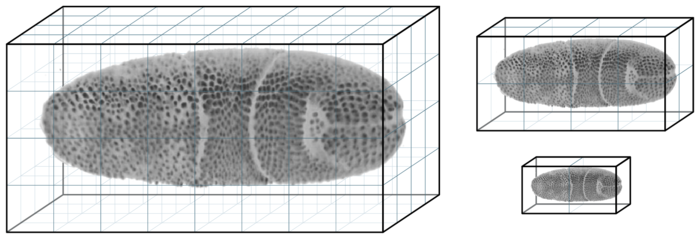
\includegraphics[width=0.6\textwidth]{figures/BdvTikz-pyramidblocks.png}
    \caption{Illustration of the BDV file format storage strategy. The image is stored over several resolution levels (multi-scale pyramid) and in chunks.}
    \label{fig:BDVchunks}
\end{figure}

There are several implementations of this strategy, for instance in Imaris\footnote{\href{http://open.bitplane.com/Default.aspx?tabid=268}{\coloredlink{IMARIS 5.5 File Format Description (IMS).}}} and with the new file format N5\footnote{\href{https://github.com/saalfeldlab/n5}{\coloredlink{N5 API on GitHub.}}} proposed by the Saalfeld lab.
Some of them are inter-compatible.
We will pick the BDV file format all along this document. 
The \Bdv has proved its value and impact on our field.
For instance our previous work on cell lineaging in large images, \wikilink{MaMuT}{MaMuT}, is based on BDV~\cite{MaMuT}.



\subsubsection{The tuturial dataset.}

Mastodon was created specially because we needed to harness very big, multi-view images. We wanted to generate  comprehensive lineages and follow a large number of cells over a very long time.
This accumulation of inflated words is tied to the very large  - in objective disk space  occupation - images we deal with using modern microscopy tools. 
Such datasets might not be optimal for a first contact with Mastodon.
So just for this tutorial we will use a smaller dataset.
It is a small region cut into a movie following the development of a drosophila, acquired in Pavel Tomancak lab (MPI-CBG).
You can find it on Zenodo\footnote{\href{https://zenodo.org/record/3336346}{\coloredlink{https://zenodo.org/record/3336346}}} there: \href{https://doi.org/10.5281/zenodo.3336346}{
\includegraphics[height=1.5\fontcharht\font`\B]{figures/zenodo3336346.png}}

It is a zip file that contains 3 files:
\begin{minted}{text}
    14M  datasethdf5.h5
   2.7K  datasethdf5.settings.xml
   8.7K  datasethdf5.xml
\end{minted}

The \texttt{.h5} file is the HDF5 file mentioned above, that contains the image data itself.
The \texttt{data\-sethdf5.xml} is a text file following the XML convention, specific to the BDV file format, that contains information about the the image data and metadata. 
When we want to open a BDV file, we point the reader to this file.
The \texttt{datasethdf5.settings.xml} is an optional file that stores user display parameters, such as channel colors, min and max display value, as well as bookmarks in the data. 
We refer you to the \wikilink{BigDataViewer\#Loading_and_Saving_Settings}{BDV documentation} about this file.
Mastodon uses this settings file to store that same information.

If you open this data in the \Bdv (in Fiji in the \menu{Plugins > BigDataViewer > Open XML/HDF5} menu), you should see something like in figure~\ref{fig:OpeningImage}. 
There is about 70 cells in each of the 30 time-points, arranged in a layer at the top of the sample. 
The deeper part of the sample (low Z coordinates) has some hazy, diffuse signal from which we cannot individualize cells.
As time progresses, the cells move towards the middle part and bottom (high Y coordinates) part of the image, and some of them move deeper in Z, initiating gastrulation.

The goal of this short tutorial is to track all these cells in Mastodon.

\begin{figure}
     \centering
         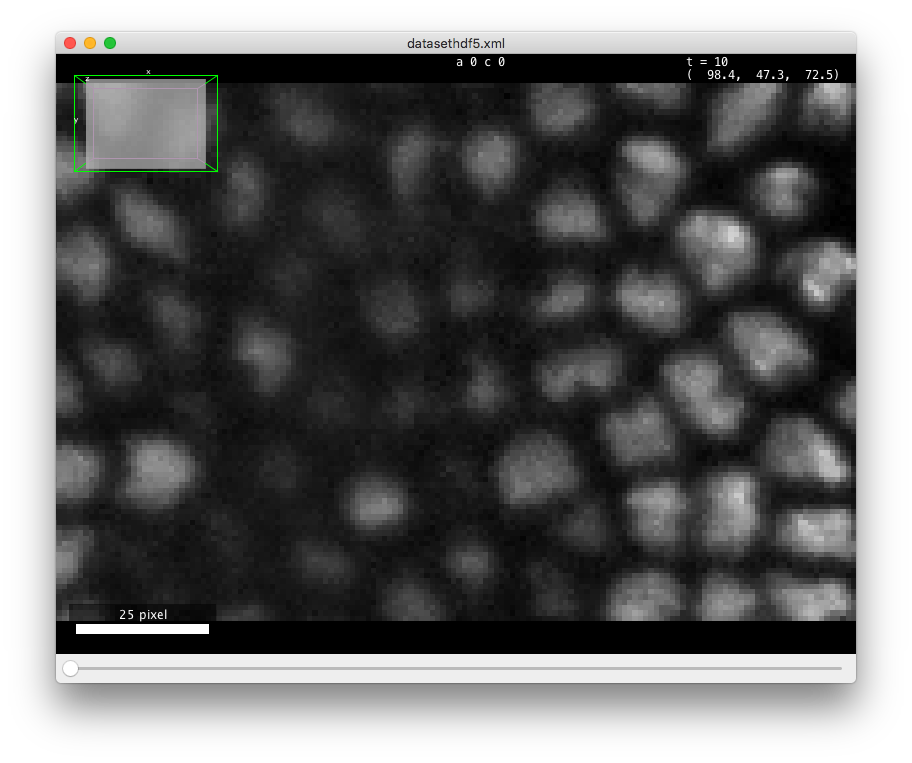
\includegraphics[width=0.3\textwidth]{figures/BDV-imageXY.png}
         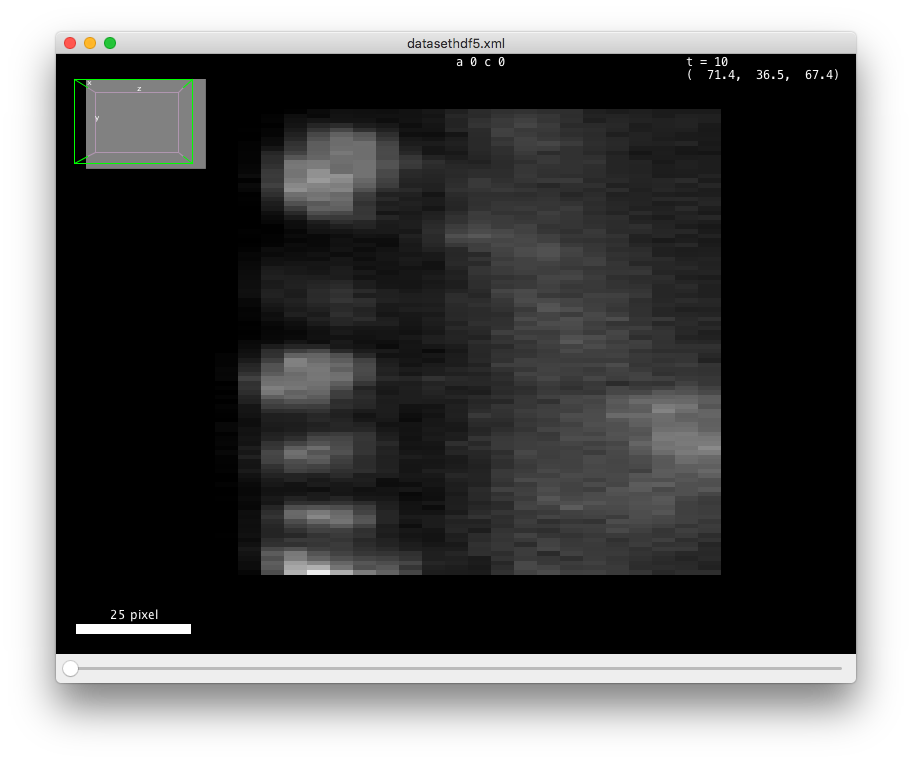
\includegraphics[width=0.3\textwidth]{figures/BDV-imageXZ.png}
         \caption{The tutorial dataset opened in \Bdv, seen along XY (left) and XZ (right)}
     \label{fig:OpeningImage}
\end{figure}  




\subsection{Getting Mastodon.}

As of today, Mastodon is available as a preview. We are still working on adding and validating features.
Nonetheless the preview has everything we need to track these cells.
Also, Mastodon is independent of ImageJ or Fiji, it can operate as a standalone software. 
However we currently distribute it via Fiji, because the updater and the dependency management are so convenient. 
So the first thing to do is to grab Fiji\footnote{\href{http://fiji.sc/}{\coloredlink{http://fiji.sc/}}}, if you do not have it already.

Then launch the \wikilink{Updater}{Fiji updater} and once your Fiji is up to date, click on the \texttt{Manage update site} button.
We will add the \wikilink{Following_an_update_site}{add the Mastodon update site}.
You should find the Mastodon preview site in the list. 
Select it, update Fiji and restart it. 
After restarting, you should find the command \menu{Plugins > Mastodon (preview)} at the bottom of the menu.

\begin{center}
    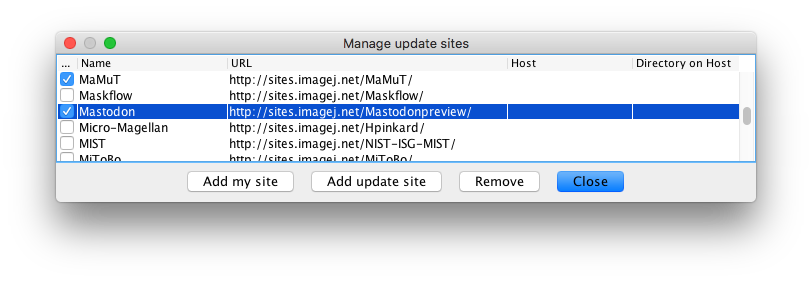
\includegraphics[width=0.7\textwidth]{figures/Mastodon_UpdateSite.png}
\end{center}



\subsection{Creating a new Mastodon project.}

After launching the command, this plain, sober window appears.
\begin{center}
         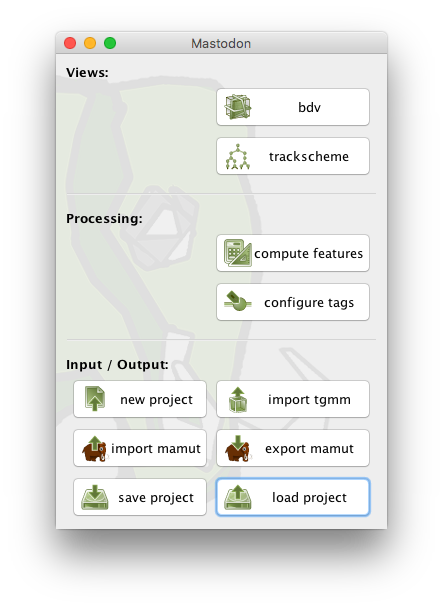
\includegraphics[width=0.3\textwidth]{figures/Mastodon_MainWindow.png}
\end{center}

Click on new \texttt{new project}, and browse to the \texttt{datasethdf5.xml} file of the XML/HDF5 file pair of the tutorial dataset.
All the buttons that were grayed out should be enabled. 
Click on the \texttt{bdv} button.
A BDV window should appear and if it does everything is right.
\begin{center}
         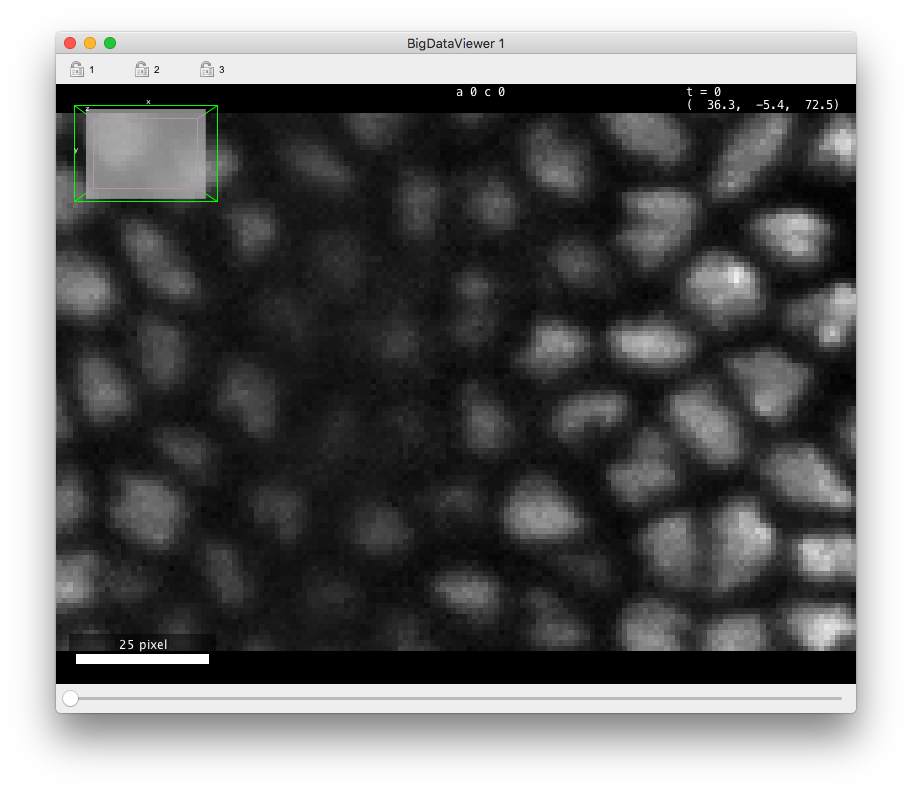
\includegraphics[width=0.4\textwidth]{figures/Mastodon_BDV.png}
\end{center}

It is almost a regular BDV window and if you already know who to use it and the key bindings you should find your marks quickly.
Below we give the commands and key-bindings for navigation in a Mastodon-BDV window. 
They are indeed close to what is found in the standard \Bdv but some changes. 
\textbf{Please note:} You can reconfigure almost everything in Mastodon, as we will see later, including key-bindings.
In this tutorial and the next ones, the key-bindings we present are for the \texttt{Default} configuration.
In the table~\ref{tab:MastodonBDVNavigationKeys} you will find the key bindings to navigate through the image data.

\begin{table}[!htbp]
    \centering
    
    \caption{Default navigation key-bindings for Mastodon-BDV views.}

    \begin{tabulary}{\textwidth}{L|J}
    
    \toprule
    \textbf{Action}                 & \textbf{Key}              
    \\ \midrule
    
    \multicolumn{2}{c}{\textit{View.}}
    \\ \midrule
    
    Move in X \& Y.                 & \keys{Right-click} and \keys{Drag}
    \\ \midrule
    
    Move in Z.                      & \keys{Mouse-wheel}. Press and hold \keys{\shift} to move faster, \keys{\ctrl} to move slower.
    \\ \midrule
    
    Align view with X / Y / Z axes. &  
    \begin{minipage}[t]{0.7\textwidth}
    \begin{itemize}
        \item  Align with XY plane: \keys{\shift+Z}
        \item Align with YZ plane: \keys{\shift+X}
        \item Align with XZ plane: \keys{\shift+C} or \keys{\shift+Y} 
    \end{itemize}
    The view will rotate around the location you clicked.
    \end{minipage}
    
    \\ \midrule
    
    Zoom / Unzoom.                  & \keys{\ctrl+\shift+Mouse-wheel} or \keys{\cmd+Mouse-wheel}. The view will zoom and unzoom around the mouse location.
    \\ \midrule

    \multicolumn{2}{c}{\textit{Time-points.}}
    \\ \midrule
    
    Next time-point.                & \keys{]} or \keys{M}
    \\ \midrule
    
    Previous time-point.            & \keys{[} or \keys{N}                                                                                     
    \\ \midrule

    \multicolumn{2}{c}{\textit{Bookmarks.}}
    \\ \midrule

    Store a bookmark.               & \keys{\shift+B} then press any key to store a bookmark with this key as name. A bookmark stores the position, zoom and orientation in the view but not the time-point. Bookmarks are saved in display settings file.
    \\ \midrule
    
    Recall a bookmark.              & Press \keys{B} then the key of the bookmark.
    \\ \midrule  
    
    Recall a bookmark orientation.  & Press \keys{O} then the key of the bookmark. Only the orientation of the bookmark will be restored.
    \\ \midrule
    
    \multicolumn{2}{c}{\textit{Image display.}}
    \\ \midrule
    
    Select source 1, 2 \ldots         & Press \keys{1} / \keys{2} \ldots
    \\ \midrule
    
    Brightness and color dialog.    & Press \keys{S}. In this dialog you can adjust the min \& max for each source, select to what sources these min \& max apply and pick a color for each source.
    \\ \midrule
    
    Toggle fused mode.              & Press \keys{F}. In fused mode, several sources are overlaid. Press \keys{\shift+1} / \keys{\shift+2} \ldots to add / remove the source to the view. In single-source mode, only one source is shown.
    \\ \midrule
    
    Visibility and grouping dialog.     & Press \keys{F6}. In this dialog you can define what sources are visible in fused mode, and define groups of sources for use in the grouping mode.
    \\ \midrule
    
    Save / load display settings.       & \keys{F11} / \keys{F12}. This will create a \texttt{XYZ\_settings.xml} file in which the display settings will be saved.
    \\ \bottomrule

\end{tabulary}


    \label{tab:MastodonBDVNavigationKeys}
    \vspace{-10pt}

\end{table}